%%%%%%%%%%%%%%%%%%%%%%%%%%%%%%%%%%%%%%%%%
% Beamer Presentation
% LaTeX Template
% Version 1.0 (10/11/12)
%
% This template has been downloaded from:
% http://www.LaTeXTemplates.com
%
% License:
% CC BY-NC-SA 3.0 (http://creativecommons.org/licenses/by-nc-sa/3.0/)
%
%%%%%%%%%%%%%%%%%%%%%%%%%%%%%%%%%%%%%%%%%

%----------------------------------------------------------------------------------------
%	PACKAGES AND THEMES
%----------------------------------------------------------------------------------------

\documentclass[handout]{beamer}

\mode<presentation> {

% The Beamer class comes with a number of default slide themes
% which change the colors and layouts of slides. Below this is a list
% of all the themes, uncomment each in turn to see what they look like.

%\usetheme{default}
%\usetheme{AnnArbor}
%\usetheme{Antibes}
%\usetheme{Bergen}
%\usetheme{Berkeley}
%\usetheme{Berlin}
%\usetheme{Boadilla}
%\usetheme{CambridgeUS}
%\usetheme{Copenhagen}
%\usetheme{Darmstadt}
%\usetheme{Dresden}
%\usetheme{Frankfurt}
%\usetheme{Goettingen}
%\usetheme{Hannover}
%\usetheme{Ilmenau}
%\usetheme{JuanLesPins}
%\usetheme{Luebeck}
\usetheme{Madrid}
%\usetheme{Malmoe}
%\usetheme{Marburg}
%\usetheme{Montpellier}
%\usetheme{PaloAlto}
%\usetheme{Pittsburgh}
%\usetheme{Rochester}
%\usetheme{Singapore}
%\usetheme{Szeged}
%\usetheme{Warsaw}

% As well as themes, the Beamer class has a number of color themes
% for any slide theme. Uncomment each of these in turn to see how it
% changes the colors of your current slide theme.

%\usecolortheme{albatross}
%\usecolortheme{beaver}
%\usecolortheme{beetle}
%\usecolortheme{crane}
%\usecolortheme{dolphin}
%\usecolortheme{dove}
%\usecolortheme{fly}
%\usecolortheme{lily}
%\usecolortheme{orchid}
%\usecolortheme{rose}
%\usecolortheme{seagull}
%\usecolortheme{seahorse}
%\usecolortheme{whale}
%\usecolortheme{wolverine}

%\setbeamertemplate{footline} % To remove the footer line in all slides uncomment this line
%\setbeamertemplate{footline}[page number] % To replace the footer line in all slides with a simple slide count uncomment this line

%\setbeamertemplate{navigation symbols}{} % To remove the navigation symbols from the bottom of all slides uncomment this line
}

\usepackage{graphicx} % Allows including images
\usepackage{booktabs} % Allows the use of \toprule, \midrule and \bottomrule in tables
\usepackage{cool}
\usepackage{tikz}
\usepackage{amsmath}
\usepackage{MnSymbol,wasysym}
\DeclareMathOperator*{\argmax}{argmax}
\DeclareMathOperator*{\argmin}{argmin}
\usetikzlibrary{positioning}

%----------------------------------------------------------------------------------------
%	TITLE PAGE
%----------------------------------------------------------------------------------------

\title[A.I For Retail/Finance]{A.I. for Dynamic Decisioning under Uncertainty} % The short title appears at the bottom of every slide, the full title is only on the title page
\subtitle{For Real-World Problems in Retail \& Financial Trading}
\author{Ashwin Rao} % Your name
\institute[Target/Stanford] % Your institution as it will appear on the bottom of every slide, may be shorthand to save space
{VP Data Science at Target \& Adjunct Faculty at Stanford
 % Your institution for the title page
}
\date{\today} % Date, can be changed to a custom date

\begin{document}
\begin{frame}
\titlepage % Print the title page as the first slide
\end{frame}

\begin{frame}
\frametitle{A.I. for Dynamic Decisioning under Uncertainty}
\pause
\begin{itemize}[<+->]
\item Let's look at some terms we use to characterize this branch of A.I.
\item {\em Stochastic}: Uncertainty in key quantities, evolving over time
\item {\em Optimization}: A well-defined metric to be maximized (``The Goal'')
\item {\em Dynamic}:  Decisions need to a function of the changing situations
\item {\em Control}: Overpower uncertainty by persistent steering towards goal
\item Jargon overload due to confluence of Control Theory, O.R. and A.I.
\item For language clarity, let's just refer to this area as {\em Stochastic Control}
\item I was introduced to this area through Inventory Control
\item At Stanford, I teach a course on \href{https://github.com/coverdrive/technical-documents/blob/master/finance/cme241/Stanford-CME241.pdf}{\underline{\textcolor{blue}{A.I. for Stochastic Control in Finance}}}
\item I'm developing an \href{https://github.com/coverdrive/MDP-DP-RL}{\underline{\textcolor{blue}{educational codebase}}} for Stochastic Control 
\item Overarching Goal: Blend Theory, Algorithms \& Real-World Modeling
\end{itemize}
\end{frame}


\begin{frame}
\frametitle{Overview} % Table of contents slide, comment this block out to remove it
\tableofcontents % Throughout your presentation, if you choose to use \section{} and \subsection{} commands, these will automatically be printed on this slide as an overview of your presentation
\end{frame}

\section{The Framework of Stochastic Control}

\begin{frame}
\frametitle{The Stochastic Control Framework}
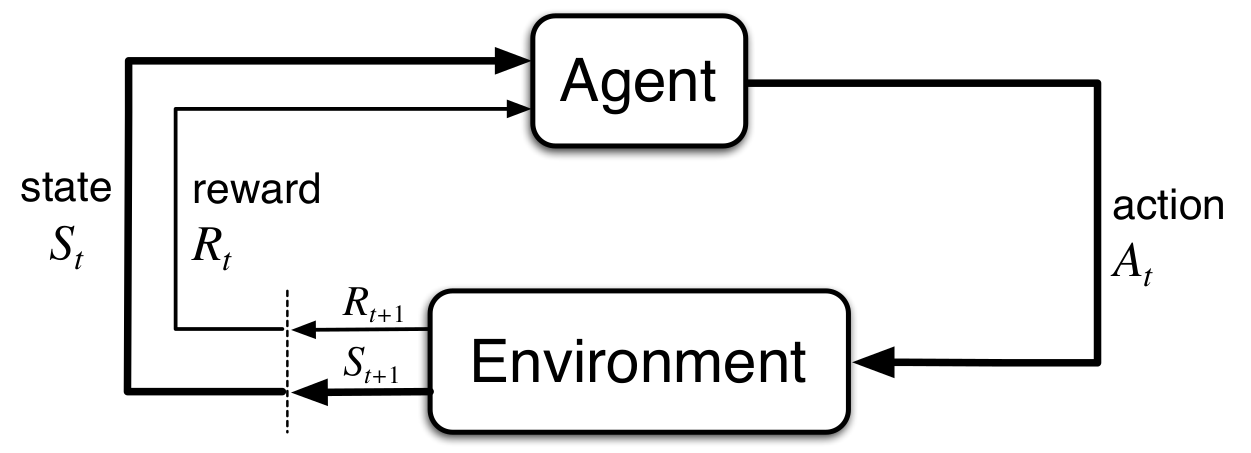
\includegraphics[width=12cm, height=7cm]{../finance/cme241/MDP.png}
\end{frame}

\begin{frame}
\frametitle{Components of the Framework}
\pause
\begin{itemize}[<+->]
\item The {\em Agent} and the {\em Environment} interact in a time-sequenced loop
\item {\em Agent} responds to [{\em State}, {\em Reward}] by taking an {\em Action}
\item {\em Environment} responds by producing next step's (random) {\em State}
\item {\em Environment} also produces a (random) number denoted as {\em Reward}
\item Goal of {\em Agent} is to maximize {\em Expected Sum} of all future {\em Reward}s
\item By controlling the ({\em Policy} : {\em State} $\rightarrow$ {\em Action}) function
\item This is a dynamic (time-sequenced control) system under uncertainty
\item Formally known as a {\em Markov Decision Process} (MDP)
\end{itemize}
\end{frame}

\begin{frame}
\frametitle{Formal MDP Framework}
\pause
The following notation is for discrete time steps. Continuous-time formulation is analogous (often involving
\href{https://github.com/coverdrive/technical-documents/blob/master/finance/cme241/StochasticCalculusFoundations.pdf}{\underline{\textcolor{blue}{Stochastic Calculus}}})
\begin{itemize}[<+->]
\item States $S_t \in \mathcal{S}$ where $\mathcal{S}$ is the State Space
\item Actions $A_t \in \mathcal{A}$ where $\mathcal{A}$ is the Action Space
\item Rewards $R_t \in \mathbb{R}$ denoting numerical feedback\
\item Transitions $p(s',r|s,a) = Pr\{S_{t+1}=s',R_{t+1}=r|S_t=s,A_t=a\}$
\item $\gamma \in [0,1]$ is the Discount Factor for Reward when defining {\em Return}
\item Return $G_t = R_t + \gamma \cdot R_{t+1} + \gamma^2 \cdot R_{t+1} + \ldots$
\item Policy $\pi(a|s)$ is probability that Agent takes action $a$ in states $s$
\item The goal is find a policy that maximizes  $\mathbb{E}[G_t|S_t = s]$ for all $s \in \mathcal{S}$
\end{itemize}
\end{frame}

\begin{frame}
\frametitle{Many real-world problems fit this MDP framework}
\pause
\begin{itemize}
\item Self-driving vehicle (speed/steering to optimize safety/time)
\item Game of Chess (Boolean {\em Reward} at end of game)
\item Complex Logistical Operations (eg: movements in a Warehouse)
\item Make a humanoid robot walk/run on difficult terrains
\item Manage an investment portfolio
\item Control a power station
\item Optimal decisions during a football game
\item Strategy to win an election (high-complexity MDP)
\end{itemize}
\end{frame}

\begin{frame}
\frametitle{Why are these problems hard?}
\pause
\begin{itemize}[<+->]
\item {\em State} space can be large or complex (involving many variables)
\item Sometimes, {\em Action} space is also large or complex
\item No direct feedback on ``correct'' {\em Actions} (only feedback is {\em Reward})
\item Time-sequenced complexity ({\em Actions} influence future {\em States/Actions})
\item {\em Action}s can have delayed consequences (late {\em Reward}s)
\item {\em Agent} often doesn't know the {\em Model} of the {\em Environment}
\item ``Model'' refers to probabilities of state-transitions and rewards
\item So, {\em Agent} has to learn the {\em Model} AND solve for the Optimal {\em Policy}
\end{itemize}
\end{frame}

\begin{frame}
\frametitle{Value Function and Bellman Equations}
\pause
\begin{itemize}
\item Value function (under policy $\pi$) $V_{\pi}(s) = \mathbb{E}[G_t|S_t = s]$ for all $s \in \mathcal{S}$
\pause
$$V_{\pi}(s) = \sum_{a} \pi(a|s) \sum_{s',r} p(s',r|s,a) \cdot (r + \gamma V_{\pi}(s')) \mbox{ for all } s \in \mathcal{S}$$
\pause
\item Optimal Value Function $V_{*}(s) = \max_{\pi} V_{\pi}(s) \mbox{ for all } s \in \mathcal{S}$
\pause
$$V_{*}(s) = \max_{a} \sum_{s',r} p(s',r|s,a) \cdot (r + \gamma V_{*}(s')) \mbox{ for all } s \in \mathcal{S}$$
\pause
\item {\em There exists an Optimal Policy} $\pi_{*}$ achieving $V_{*}(s)$ for all $s \in \mathcal{S}$
\pause
\item Determining $V_{\pi}(s)$ known as {\em Prediction}, and $V_{*}(s)$ known as {\em Control}
\pause
\item The above recursive equations are called {\em Bellman equations}
\pause
\item In continuous time, refered to as {\em Hamilton-Jacobi-Bellman (HJB)}
\pause
\item The algorithms based on Bellman equations are broadly classified as:
\begin{itemize}
\item Dynamic Programming
\item Reinforcement Learning
\end{itemize}

\end{itemize}
\end{frame}


\begin{frame}
\frametitle{Dynamic Programming versus Reinforcement Learning}
\pause
\begin{itemize}[<+->]
\item When Model is known $\Rightarrow$ {\em Dynamic Programming} (DP)
\item DP Algorithms take advantage of knowledge of probabilities
\item So, DP Algorithms do not require interaction with the environment
\item Model-based/DP algorithms often refered to as {\em Planning Algorithms}
\item When Model is unknown $\Rightarrow$ {\em Reinforcement Learning} (RL)
\item RL Algorithms interact with the Environment and incrementally learn
\item Environment interaction could be real interaction or a simulator
\item RL approach: Try different actions \& learn what works, what doesn't
\item RL Algorithms' key challenge is to tradeoff ``explore'' versus ``exploit''
\item DP or RL, Good approximation of Value Function is vital to success
\item Deep Neural Networks are typically used for function approximation
\end{itemize}
\end{frame}


\section{Core Problem in Retail: Inventory Control}

\begin{frame}
\frametitle{Inventory Control starts with the Newsvendor Problem}
\pause
\begin{itemize}[<+->]
\item Newsvendor problem is a single-period Inventory Control problem
\item Daily demand for newspapers is a random variable $x$
\item The newsvendor has an estimate of the PDF $f(x)$ of daily demand
\item For each newspaper that stays unsold, we suffer an {\em Excess cost} $h$
\item Think of $h$ as the purchase price minus salvage price
\item For each newspaper we're short on, we suffer a {\em Deficit Cost} $p$
\item Think of $p$ as the missed profits (sale price minus purchase price)
\item But $p$ should also include potential loss of future customers
\item What is the optimum \# of newspapers to bring in the morning?
\item To minimize the expected cost (function of $f$, $h$ and $p$)
\end{itemize}
\end{frame}

\begin{frame}
\frametitle{The Newsvendor Problem}
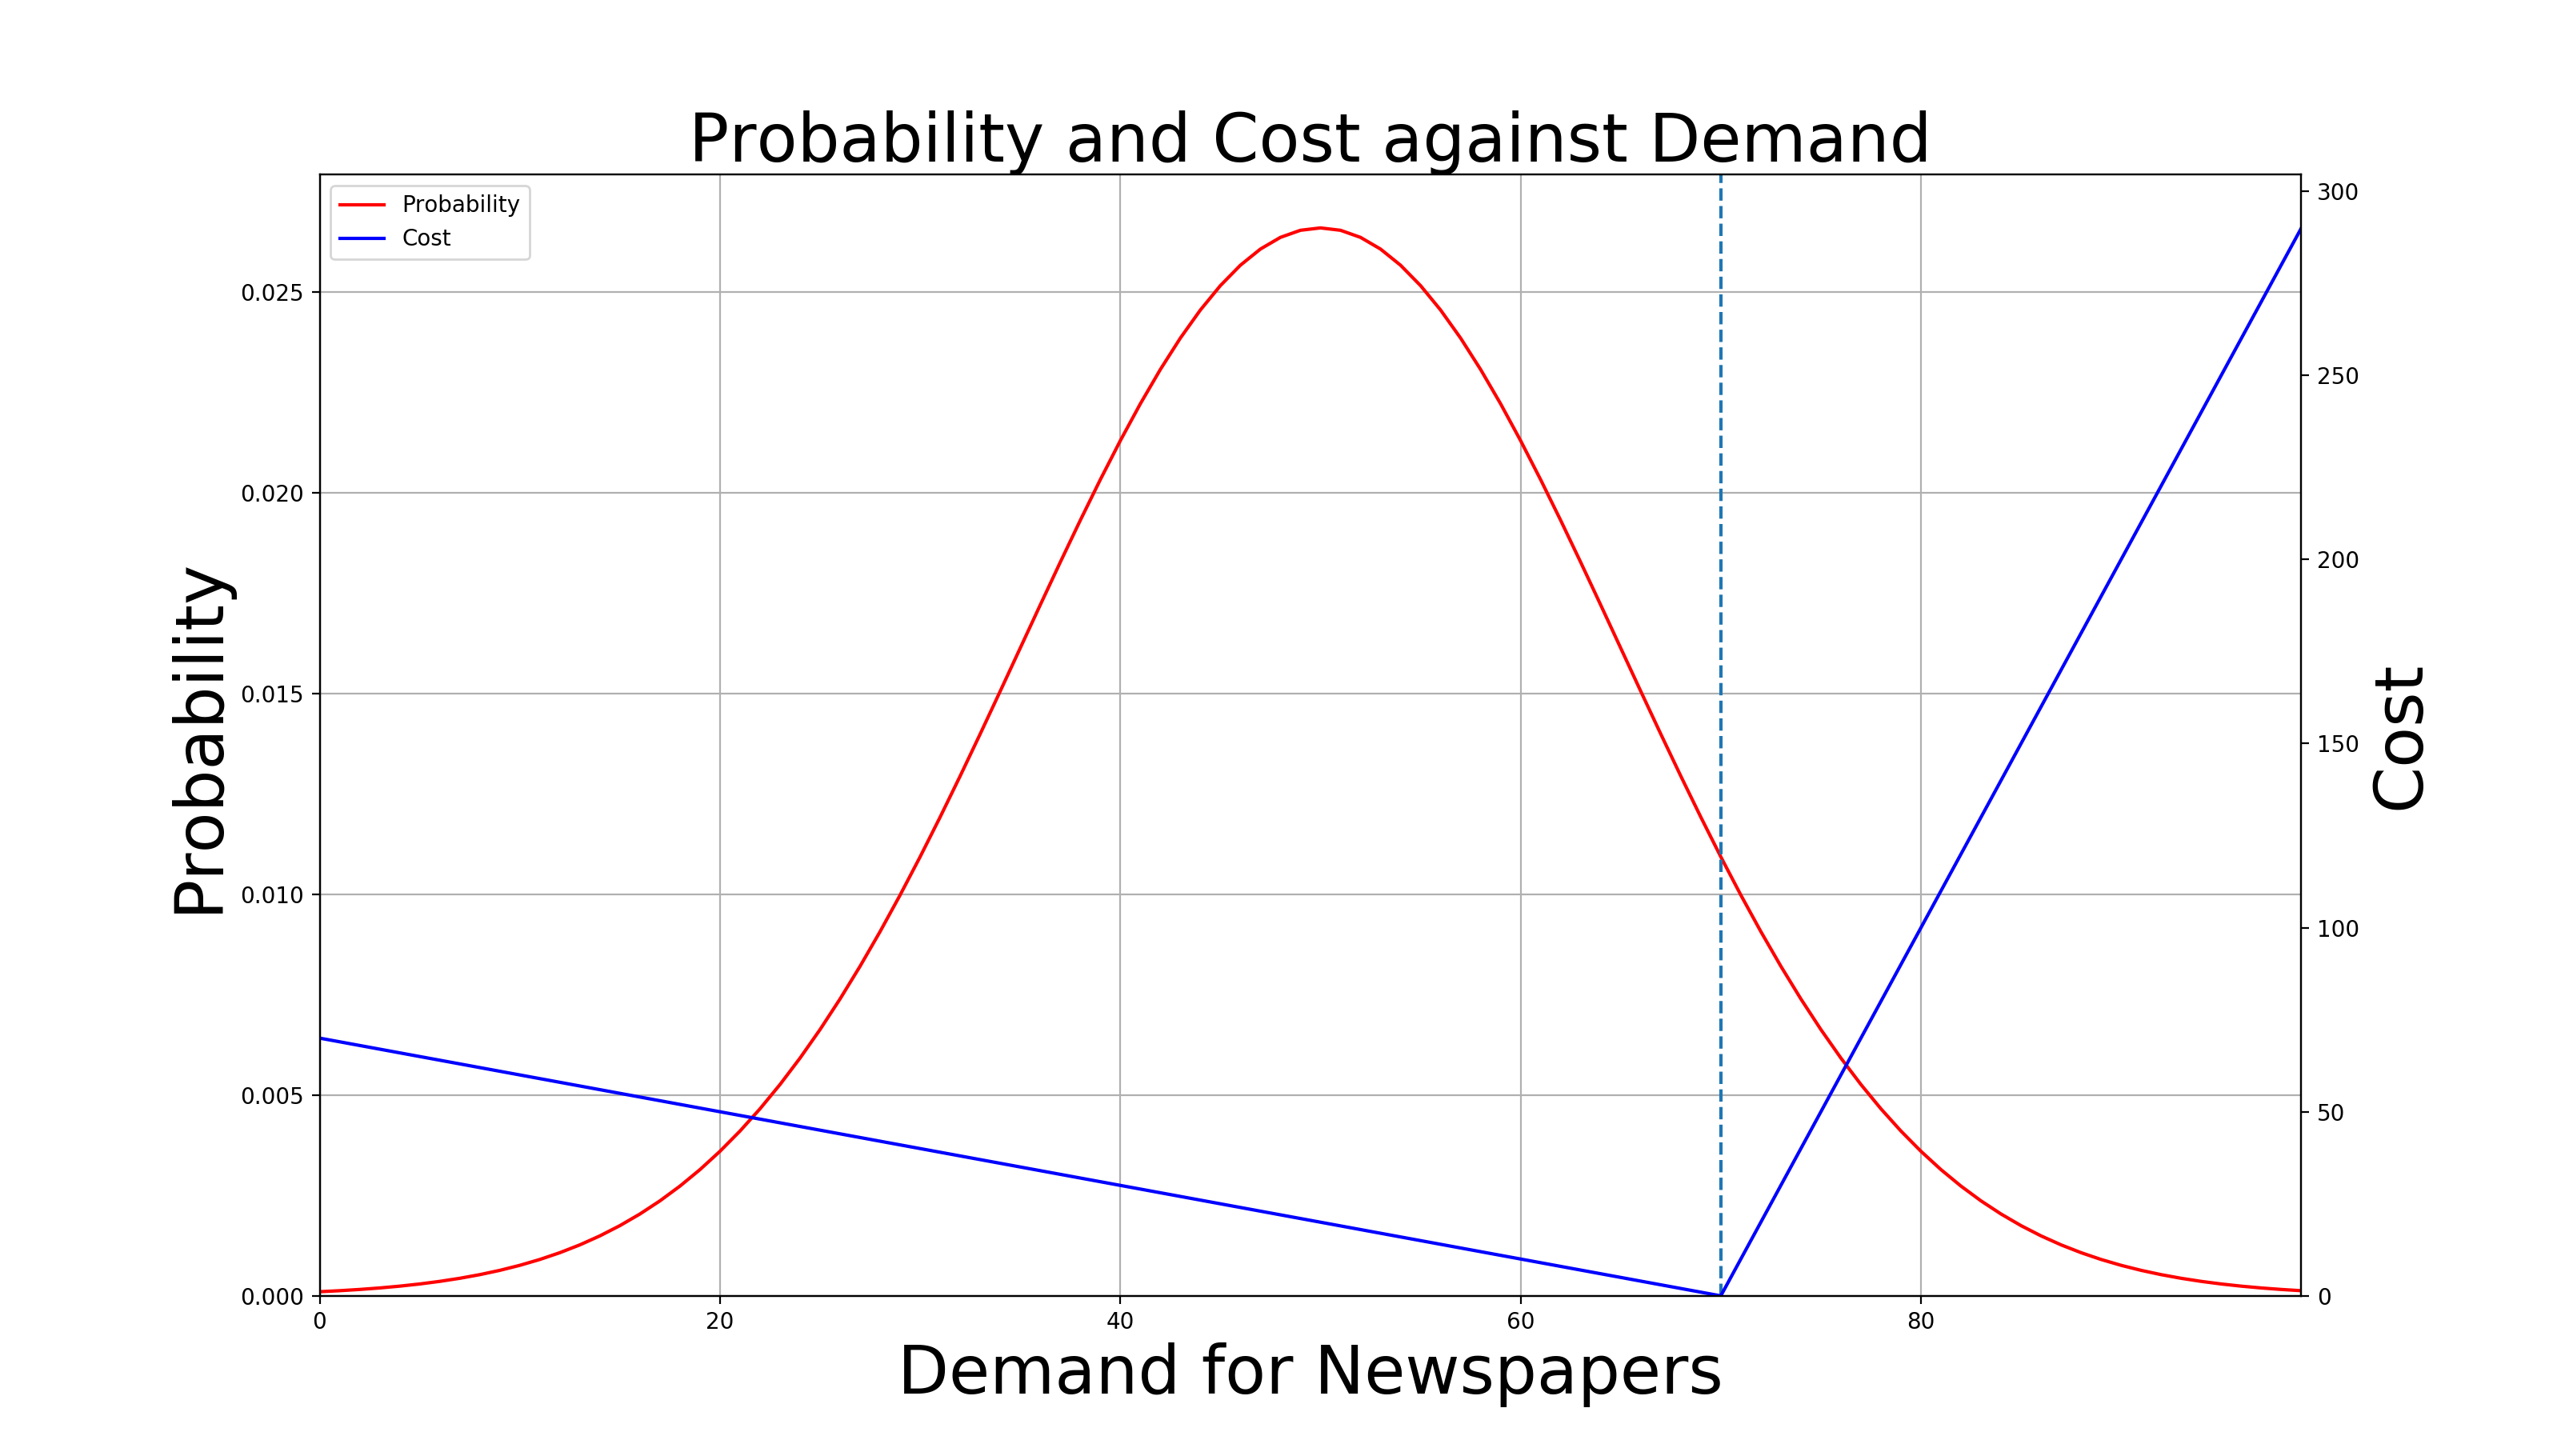
\includegraphics[width=12cm, height=8cm]{newsvendor.png}
\end{frame}

\begin{frame}
\frametitle{Solution to the Newsvendor problem}
\pause
\begin{itemize}[<+->]
\item For tractability, we assume newspapers are a continuous variable $x$
\item Then, we need to solve for the optimal supply $S$ that maximizes
$$g(S) = h \int_0^S (S-x) \cdot f(x) \cdot dx + p \int_S^{\infty} (x-S) \cdot f(x) \cdot dx$$
\item Setting $g'(S) =0$, we get:
$$\mbox{ Optimal Supply } S^* = F^{-1}(\frac p {p+h})$$
where $F(y) = \int_0^y f(x) dx$ is the CDF of daily demand
\item $\frac p {p+h}$ is known as the critical fractile
\item It is the fraction of days when the newsvendor goes ``out-of-stock''
\item Assuming the newsvendor always brings this optimal supply $S^*$
\item Solution details and connections with Financial Options Pricing \href{https://github.com/coverdrive/technical-documents/blob/master/supply_chain/NewsvendorOptionsPricing/NewsvendorOptionsPricing.pdf}{\underline{\textcolor{blue}{here}}}
\end{itemize}
\end{frame}

\begin{frame}
\frametitle{Multi-period: Single-store, Single-item Inventory Control}
\pause
\begin{itemize}[<+->]
\item The store experiences random daily demand given by PDF $f(x)$
\item The store can order daily from a supplier carrying infinite inventory
\item There's a cost associated with ordering, and order arrives in $L$ days
\item Like newsvendor, there's an Excess Cost $h$ and Deficit Cost $p$
\item This is an MDP where {\em State} is current Inventory Level at the store
\item {\em State} also includes current in-transit inventory (from supplier)
\item {\em Action} is quantity to order in any given {\em State}
\item {\em Reward} function has $h$, $p$ (just like newsvendor), and ordering cost
\item Transition probabilities are governed by demand distribution $f(x)$
\item This has a closed-form solution, similar to newsvendor fomula
\end{itemize}
\end{frame}

\begin{frame}
\frametitle{Optimal Policy: Order Point and Order-Up-To Level}
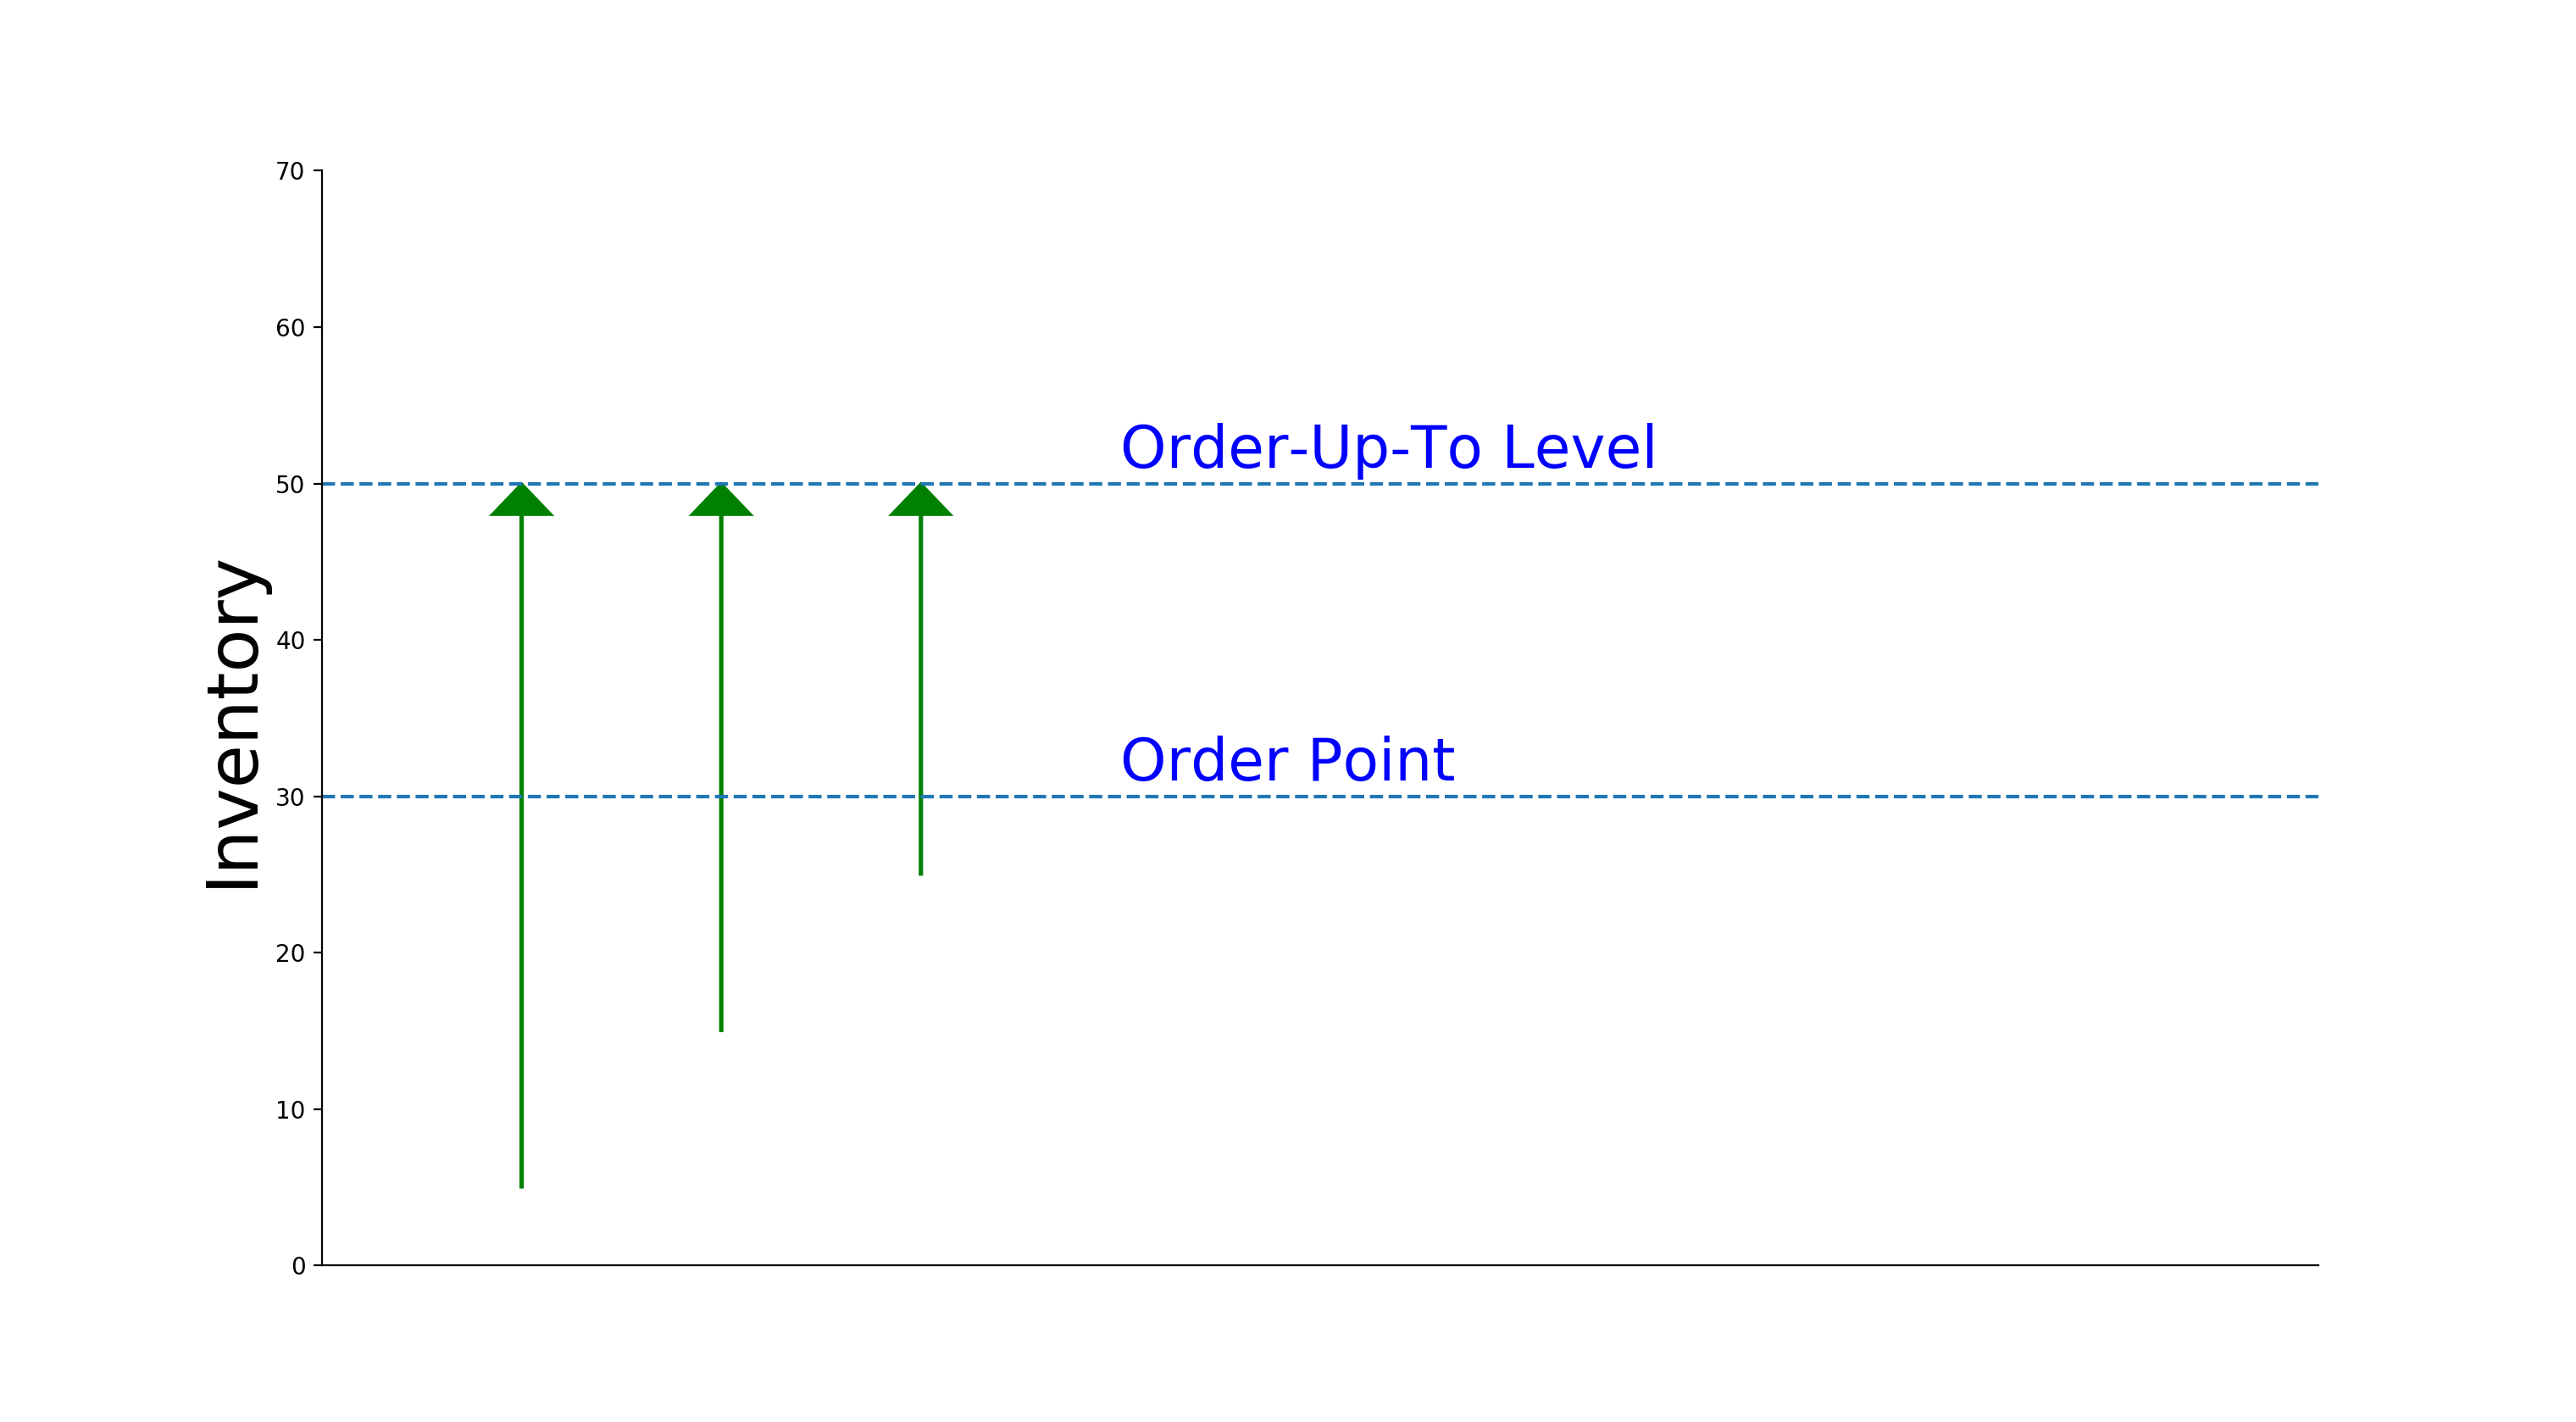
\includegraphics[width=12.5cm, height=8.5cm]{op_otl.png}
\end{frame}

\begin{frame}
\frametitle{Adding real-world frictions and constraints}
\pause
\begin{itemize}[<+->]
\item Inventory is integer-valued, and orders are in casepack units
\item Excess/Deficit costs are not linear functions of inventory
\item Perishability, Obsolescence, End-of-season involve big costs 
\item Need to factor in labor costs of handling cases and singles
\item Limits on shipping/receiving dates/times
\item Often, there is a constraint on minimum presentation quantities
\item Store inventory cannot exceed a threshold (eg: Shelf space)
\item Supplier has constraints on min and max order quantities
\item Uncertainty with the time for order arrival
\item There are approximate closed-form solutions in some cases
\item But general case requires generic DP or RL Algorithms
\end{itemize}
\end{frame}

\begin{frame}
\frametitle{Multi-node and Multi-item Inventory Control}
\pause
\begin{itemize}[<+->]
\item In practice, Inventory flows through a network of warehouses
\item From source (suppliers) to destination (stores or homes)
\item So, we have to solve a multi-``node'' Inventory Control problem
\item {\em State} is joint inventory across all nodes (and between nodes)
\item {\em Action} is recommended movements of inventory between nodes
\item {\em Reward} is the aggregate of daily costs across the network
\item In addition, we have multi-item constraints
\item Space and Throughput constraints are multi-item constraints
\item So, real-world problem is multi-node and multi-item (giant MDP)
\end{itemize}
\end{frame}

\section{Core Problem in Finance: Portfolio Optimization/Asset Allocation}

\begin{frame}
\frametitle{Single-period Portfolio Optimization}
\pause
\begin{itemize}[<+->]
\item We start with a simple single-period portfolio optimization problem
\item The simple setup helps develop understanding of the core concepts
\item Assume we have one risky asset and one riskless asset
\item The return (over the single-period) of the risky asset is $\mathcal{N}(\mu, \sigma^2)$
\item The return of the riskless asset is deterministic ($=r < \mu$)
\item Start with \$1, aim to maximize our period-ending Expected Wealth
\item This means we invest fully in the risky asset (since $\mu > r$)
\item But people are risk-averse and will trade higher returns for lower risk
\item The exact Risk-Return tradeoff is specified through {\em Utility of Wealth}
\item {\em Utility} is a concave function of Wealth describing {\em Risk-Aversion}
\item For an intro to Risk-Aversion and Utility Theory, \href{https://github.com/coverdrive/technical-documents/blob/master/finance/cme241/UtilityTheoryForRisk.pdf}{\underline{\textcolor{blue}{see here}}}
\item The goal is to maximize period-ending {\bf Expected Utility of Wealth}
\end{itemize}
\end{frame}

\begin{frame}
\frametitle{Concave Utility of Consumption $\Rightarrow \mathbb{E}[U(x)] < U(\mathbb{E}[x])$}
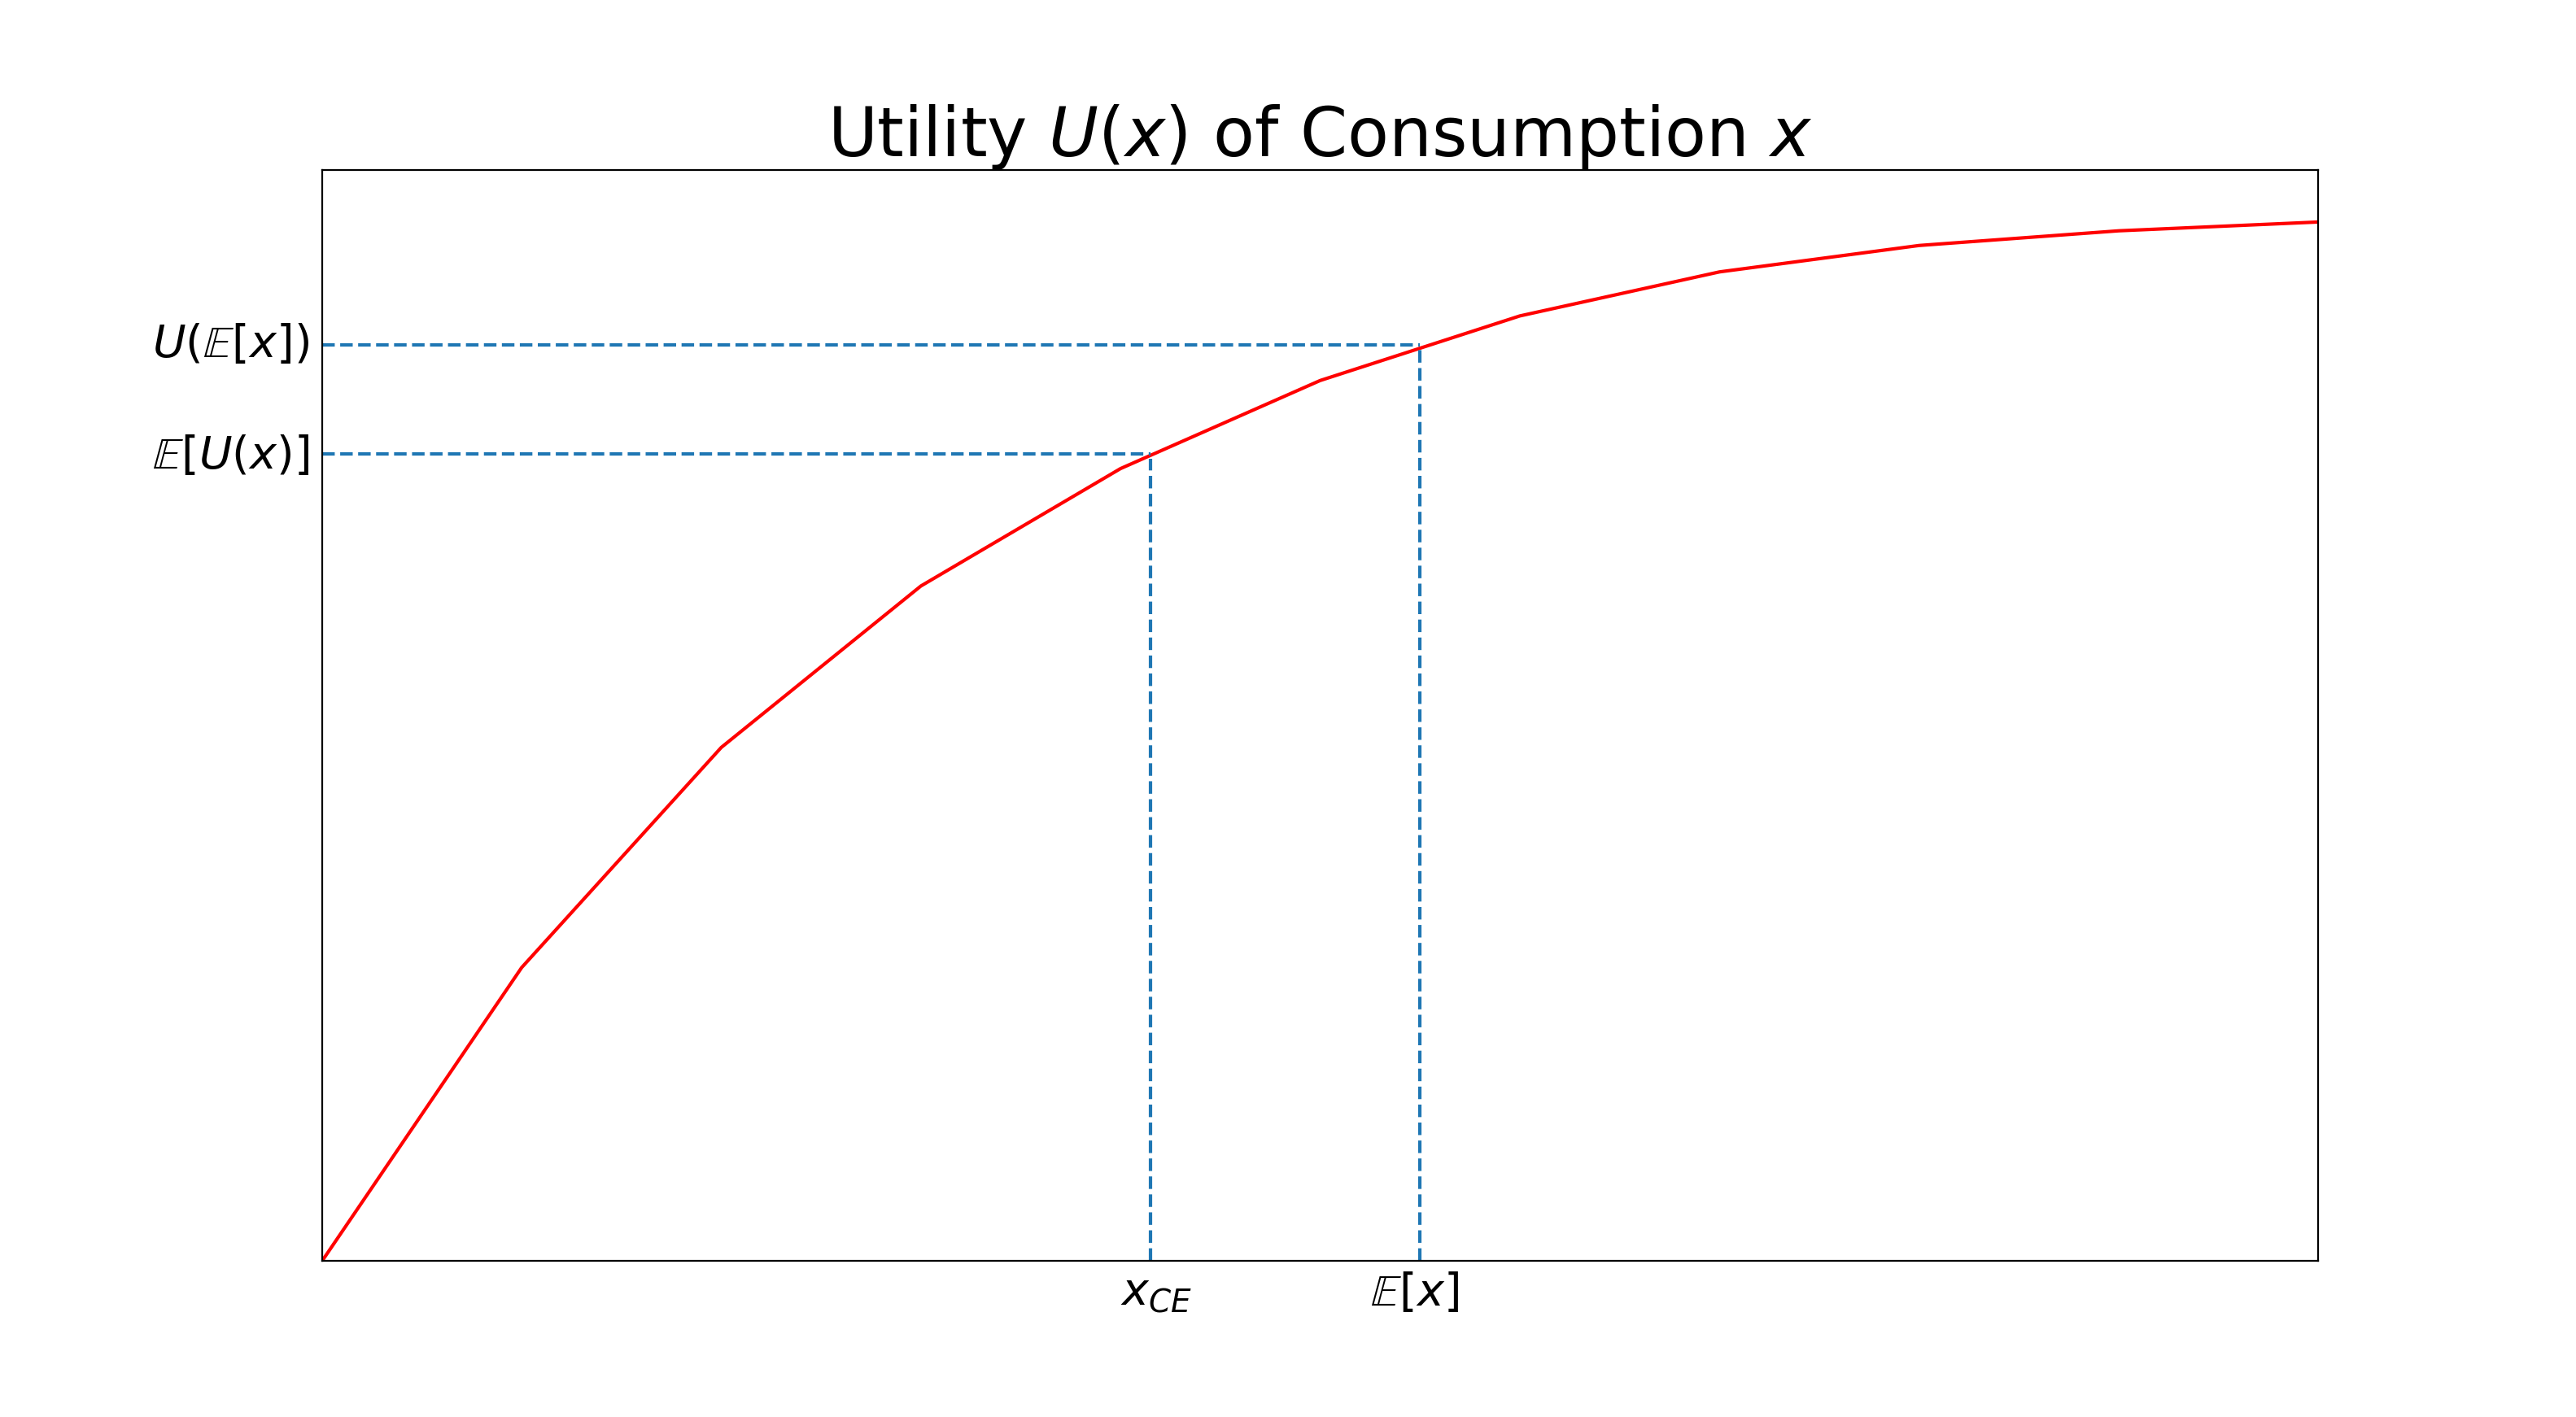
\includegraphics[scale=0.32]{ce.png}
\end{frame}

\begin{frame}
\frametitle{Solution to Single-period Portfolio Optimization}
\pause
\begin{itemize}[<+->]
\item $W$ denotes end-of-period Wealth
\item $\alpha$ denotes fraction to invest in risky asset ($1-\alpha$ is fraction in riskless)
$$W \sim \mathcal{N}(1 + r + \alpha(\mu - r), \alpha^2 \sigma^2)$$
\item Let Utility of Wealth function be $U(W) = -e^{-\beta W}$ for $\beta > 0$
\item Where $\beta$ is the coefficient (extent) of Risk-Aversion
\item So we maximize over $\alpha$, the Expected Utility
$$\mathbb{E}[-e^{-\beta W}] = -e^{-\beta(1 + r + \alpha(\mu - r)) + \frac {\beta^2 \alpha^2 \sigma^2} 2} = g(\alpha)$$
\item Setting $\pderiv{\{\log{g(\alpha)}\}}{\alpha} = 0$, we get:
$$\alpha^* = \frac {\mu - r} {\beta \sigma^2}$$
\item This is the fundamental investment fraction in Portfolio Optimization
\item This fraction generalizes to multi-period and multiple risky assets
\end{itemize}
\end{frame}

\begin{frame}
\frametitle{Multi-Period: Merton's Portfolio Optimization Problem}
\pause
\begin{itemize}[<+->]
\item You will live for (deterministic) $T$ more years (say 20 years)
\item Current Wealth is $W_0 $ (say \$ 10 million)
\item Assume you have no further income and no debts
\item You can invest in (allocate to) $n$ risky assets and a riskless asset
\item Each asset has known normal distribution of returns
\item Allowed to long or short any fractional quantities of assets
\item Trading in continuous time $0 \leq t < T$, with no transaction costs
\item You can consume any fractional amount of wealth at any time
\item Dynamic Decision: Optimal Allocation and Consumption at each time
\item To maximize lifetime-aggregated Utility of Consumption
\item Consumption Utility assumed to have constant Relative Risk-Aversion
\end{itemize}
\end{frame}

\begin{frame}
\frametitle{Problem Notation}
\pause
For ease of exposition, we state the problem for 1 risky asset
\pause
\begin{itemize}[<+->]
\item Riskless asset: $dR_t = r \cdot R_t \cdot dt$
\item Risky asset: $dS_t = \mu \cdot S_t \cdot dt + \sigma \cdot S_t \cdot dz_t$ (i.e. Geometric Brownian)
\item $\mu > r > 0, \sigma > 0$ (for $n$ assets, we work with a covariance matrix)
\item Wealth at time $t$ is denoted by $W_t > 0$
\item Fraction of wealth allocated to risky asset denoted by $\pi(t, W_t)$
\item Fraction of wealth in riskless asset will then be $1 - \pi(t, W_t)$
\item Wealth consumption denoted by $c(t, W_t) \geq 0$
\item Utility of Consumption function $U(x) = \frac {x^{1-\beta}} {1 - \beta}$ for $0 < \beta \neq 1$
\item $\beta =$ (constant) Relative Risk-Aversion $\frac {-x \cdot U''(x)} {U'(x)}$
\end{itemize}
\end{frame}

\begin{frame}
\frametitle{Continuous-Time Stochastic Control Problem}
\pause
\begin{itemize}[<+->]
\item Balance constraint implies the following process for Wealth $W_t$
$$dW_t = ((\pi_t \cdot (\mu - r) + r) \cdot W_t - c_t) \cdot dt + \pi_t \cdot \sigma \cdot W_t \cdot dz_t$$
\item At any time $t$, determine optimal $[\pi(t,W_t), c(t, W_t)]$ to maximize:
$$E[\int_t^T \frac {\gamma^{s-t} \cdot c_s^{1-\beta}} {1-\beta} \cdot ds \mid W_t]$$
\item where $0 \leq \gamma \leq 1$ is the annualized discount factor
\item Think of this as a continuous-time Stochastic Control problem
\item {\em State} is $(t, W_t)$, {\em Action} is $[\pi_t, c_t]$, {\em Reward} per unit time is $U(c_t)$
\item Stochastic process for $W_t$ above defines the transition probabilities
\item Find {\em Policy} $: (t, W_t) \rightarrow [\pi_t, c_t]$ that maximizes the {\em Expected Return}
\item Note: $c_t \geq 0$, but $\pi_t$ is unconstrained
\end{itemize}
\end{frame}


\begin{frame}
\frametitle{Outline of Solution}
\pause
\begin{itemize}[<+->]
\item Optimal Value Function $V^*(t, W_t)$ has a recursive formulation
$$V^*(t, W_t) = \max_{\pi, c} E[\int_t^{t_1} \frac {\gamma^s \cdot c_s^{1-\beta}} {1 - \beta} \cdot ds + V^*(t_1, W_{t_1})]$$
\item Re-expressed as a Hamilton-Jacobi-Bellman (HJB) formulation
$$\max_{\pi_t, c_t} E[dV^*(t, W_t) + \frac {\gamma^t \cdot c_t^{1-\beta}}{1 - \beta} \cdot dt] = 0$$
\item Standard HJB calculus (Ito's Lemma followed by partial derivatives w.r.t. $\pi_t, c_t$) gives us a PDE for $V^*(t, W_t)$
\item We can reduce the PDE to a tractable ODE with a guessed solution
\item All the gory details in \href{https://github.com/coverdrive/technical-documents/blob/master/finance/cme241/MertonPortfolio.pdf}{\underline{\textcolor{blue}{this lecture}}}
\item This solution outline is broadly applicable to continuous-time problems
\end{itemize}
\end{frame}

\begin{frame}
\frametitle{Gaining Insights into the Solution}
\begin{itemize}
\item Optimal Allocation $\pi^*(t, W_t) = \frac {\mu - r} {\sigma^2 \beta}$ (independent of $t$ and $W_t$)
\item Optimal Fractional Consumption $\frac {c^*(t, W_t)} {W_t}$ depends only on $t$ ($= f(t)$)
\item With Optimal Allocation \& Consumption, the Wealth process is:
$$\frac {dW_t} {W_t} = (r + \frac {(\mu - r)^2} {\sigma^2 \beta} - f(t)) \cdot dt + \frac {\mu - r} {\sigma \beta} \cdot dz_t$$
\item Expected Portfolio Return is constant over time ($=r + \frac {(\mu - r)^2} {\sigma^2 \beta}$)
\item Fractional Consumption $f(t)$ increases over time
\item Expected Rate of Wealth Growth $r + \frac {(\mu - r)^2} {\sigma^2 \beta} - f(t)$ decreases over time
\item If $r + \frac {(\mu - r)^2} {\sigma^2 \beta} > f(0)$, we start by Consuming $<$ Expected Portfolio Growth and over time, we Consume $>$ Expected Portfolio Growth
\item Wealth Growth Volatility is constant ($= \frac {\mu - r} {\sigma \beta}$)
\end{itemize}
\end{frame}

\begin{frame}
\frametitle{Portfolio Return versus Consumption Rate}
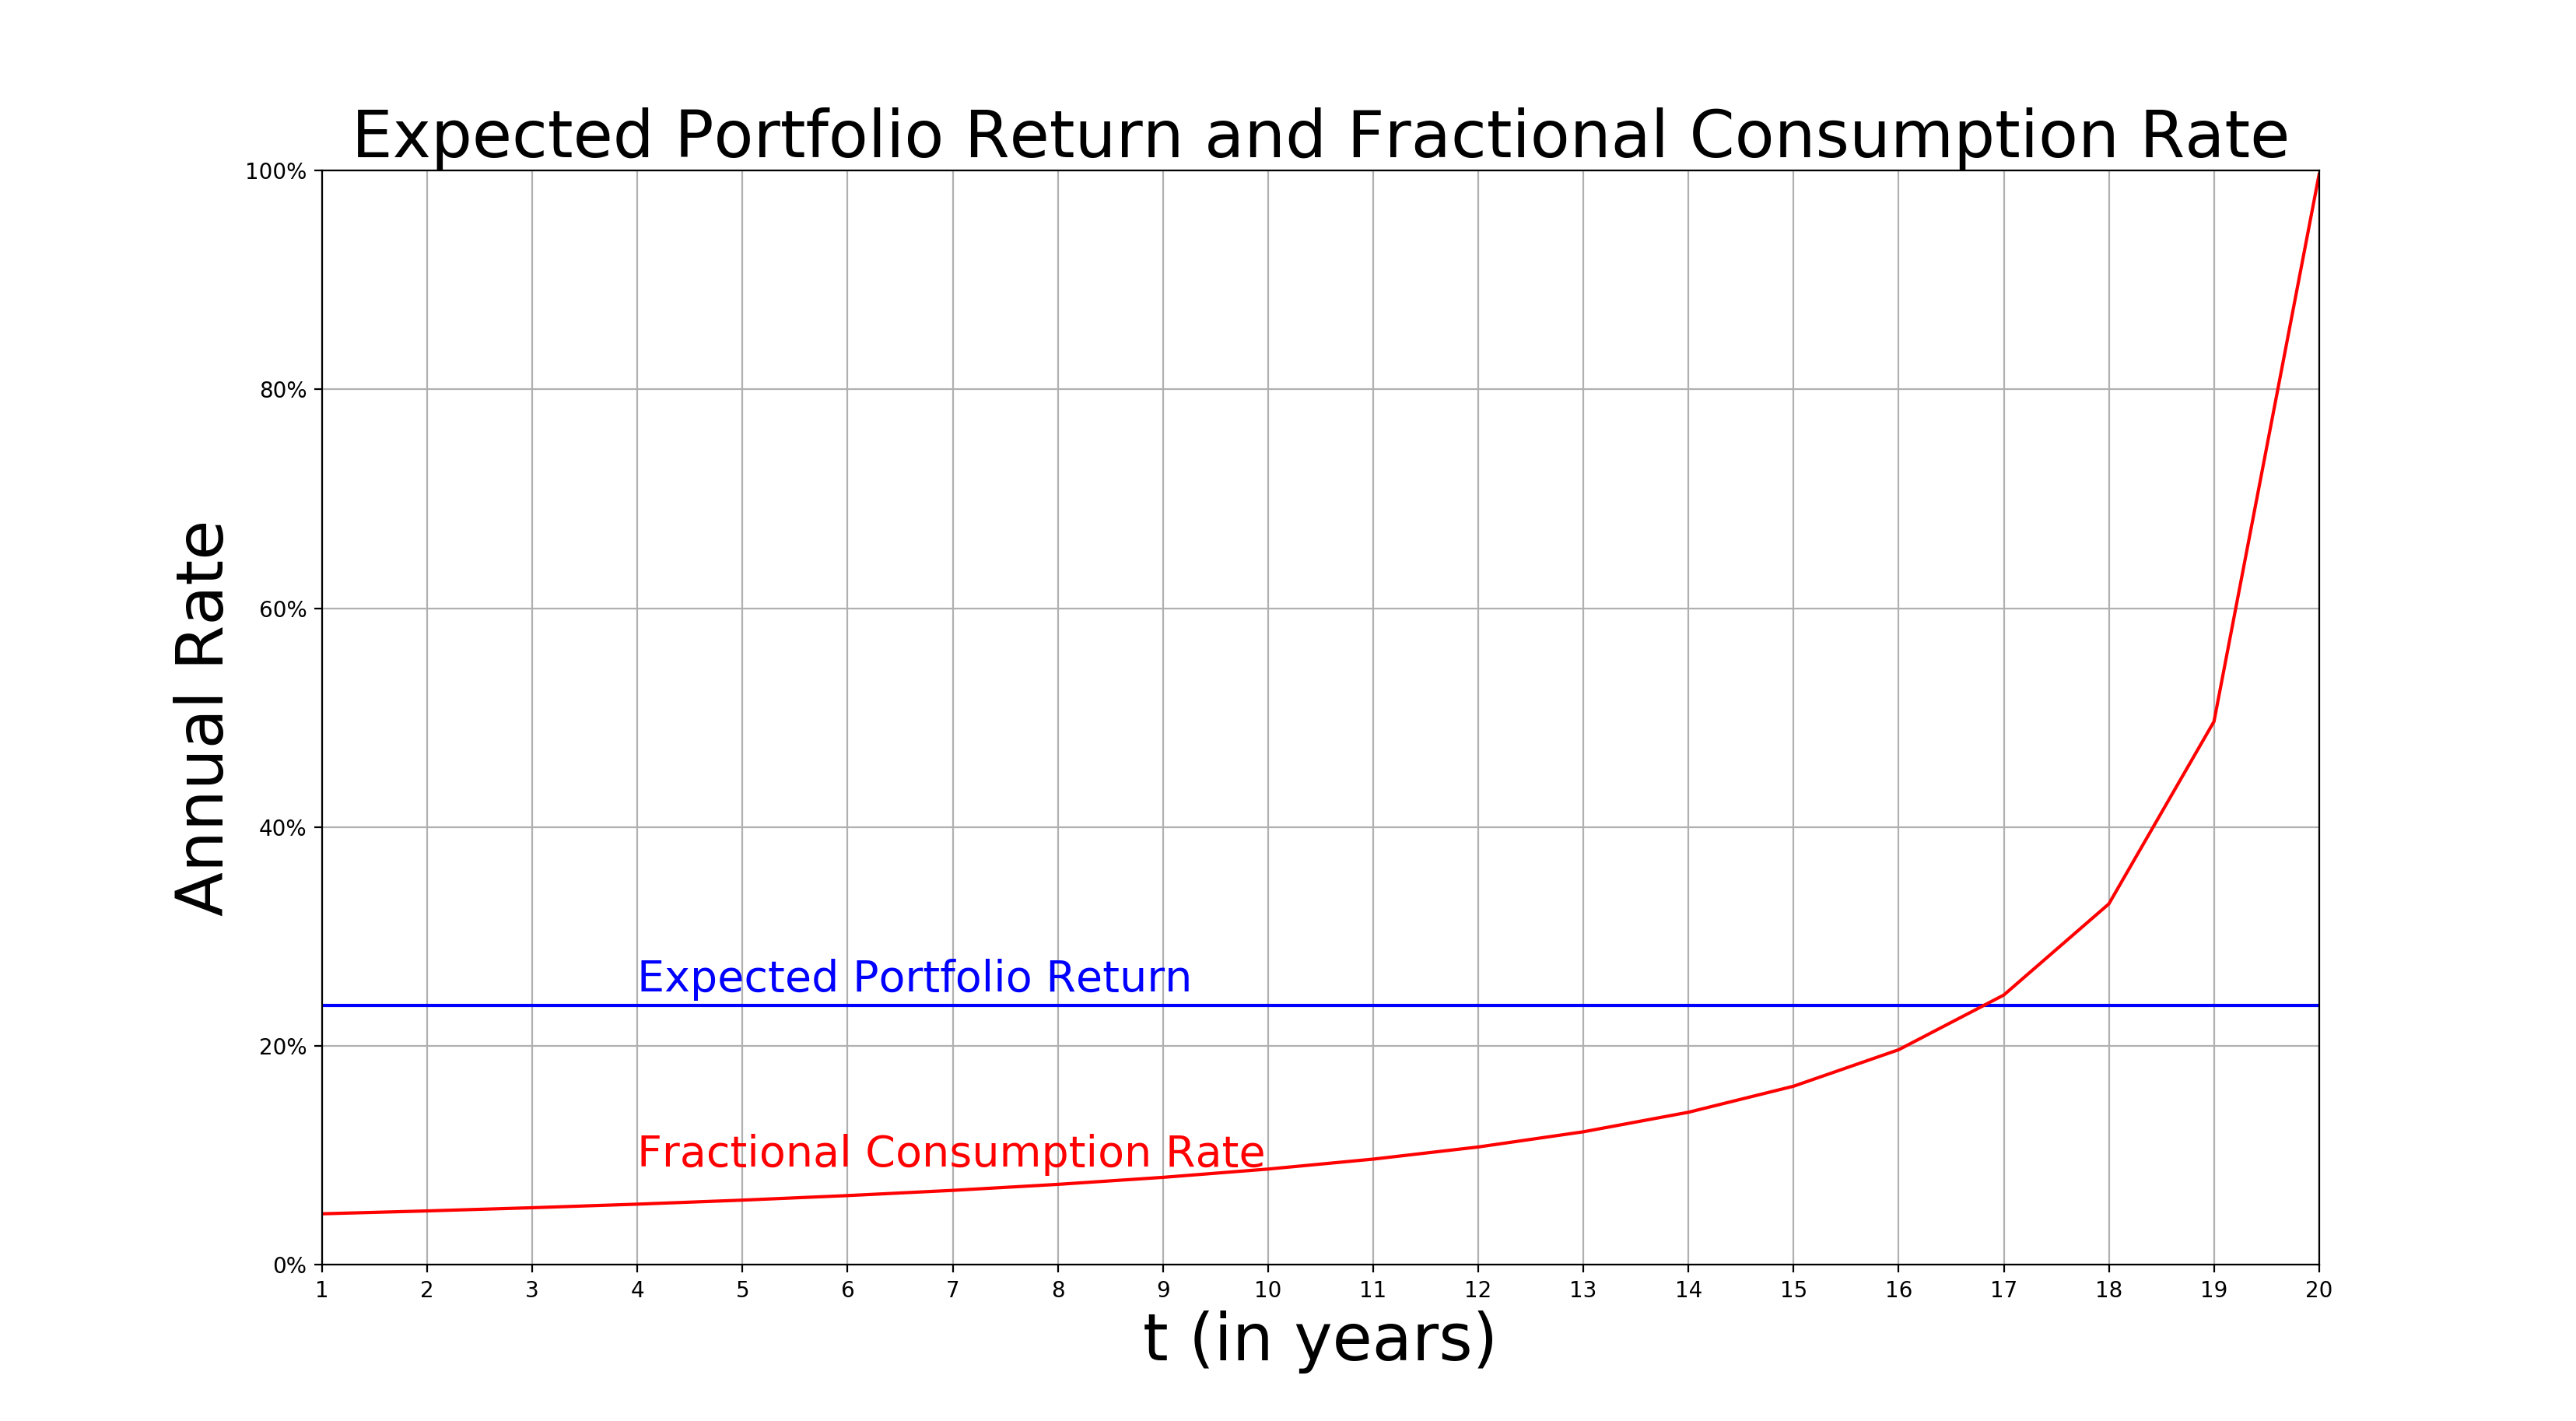
\includegraphics[width=12cm, height=8cm]{portfolio.png}
\end{frame}


\begin{frame}
\frametitle{Porting this to Real-World Portfolio Optimization}
\pause
\begin{itemize}[<+->]
\item Analytical tractability in Merton's formulation was due to:
\begin{itemize}
\item Normal distribution of asset returns
\item Constant Relative Risk-Aversion
\item Frictionless, continuous trading
\end{itemize}
\item However, real-world situation involves:
\begin{itemize}
\item Discrete amounts of assets to hold and discrete quantities of trades
\item Transaction costs
\item Locked-out days for trading
\item Non-stationary/arbitrary/correlated processes of multiple assets
\item Changing/uncertain risk-free rate
\item Consumption constraints
\item Arbitrary Risk-Aversion/Utility specification
\end{itemize}
\item $\Rightarrow$ Approximate Dynamic Programming or Reinforcement Learning
\item Large Action Space points to Policy Gradient Algorithms
\end{itemize}
\end{frame}

\section{Quick look at a few other problems in Retail and Finance}

\begin{frame}
\frametitle{Overview of a few other problems}
\begin{itemize}
\item Financial Trading: American Options Pricing
\item Financial Trading: Trade Order Execution
\item Retail: Clearance Pricing 
\end{itemize}
\end{frame}

\begin{frame}
\frametitle{American Options Pricing}
\pause
\begin{itemize}[<+->]
\item American option can be exercised anytime before option maturity
\item Key decision at any time is to exercise or continue
\item The default algorithm is Backward Induction on a tree/grid
\item But it doesn't work for path-dependent options 
\item Also, it's not feasible when state dimension is large
\item Industry-Standard: Longstaff-Schwartz's simulation-based algorithm
\item RL is an attractive alternative to Longstaff-Schwartz
\item RL is straightforward once Optimal Exercise is modeled as an MDP
\end{itemize}
\end{frame}

\begin{frame}
\frametitle{MDP for Optimal Options Exercise}
\pause
\begin{itemize}
\item {\em State} is [Current Time, History of Underlying Security Prices]
\item {\em Action} is Boolean: Exercise (i.e., Payoff and Stop) or Continue
\item {\em Reward} always 0, except upon Exercise ($=$ Payoff)
\item {\em State}-transitions governed by Underlying Prices' Stochastic Process
\item Optimal Policy $\Rightarrow$ Optimal Stopping $\Rightarrow$ Option Price
\item All the details in \href{https://github.com/coverdrive/technical-documents/blob/master/finance/cme241/AmericanOptionsRL.pdf}{\underline{\textcolor{blue}{this lecture}}}
\item Can be generalized to other Optimal Stopping problems
\end{itemize}
\end{frame}

\begin{frame}
\frametitle{Optimal Trade Order Execution (controlling Price Impact)}
\pause
\begin{itemize}[<+->]
\item You are tasked with selling a large qty of a (relatively less-liquid) stock
\item You have a fixed horizon over which to complete the sale
\item The goal is to maximize aggregate sales proceeds over the horizon
\item If you sell too fast, {\em Price Impact} will result in poor sales proceeds
\item If you sell too slow, you risk running out of time
\item We need to model temporary and permanent {\em Price Impact}s
\item Objective should incorporate penalty for variance of sales proceeds
\item Which is equivalent to maximizing aggregate Utility of sales proceeds 
\end{itemize}
\end{frame}

\begin{frame}
\frametitle{MDP for Optimal Trade Order Execution}
\pause
\begin{itemize}
\item {\em State} is [Time Remaining, Stock Remaining to be Sold, Market Info]
\item {\em Action} is Quantity of Stock to Sell at current time
\item {\em Reward} is Utility of Sales Proceeds (i.e., Variance-adjusted-Proceeds)
\item {\em Reward} \& {\em State}-transitions governed by {\em Price Impact Model}
\item Real-world {\em Model} can be quite complex (Order Book Dynamics)
\end{itemize}
\end{frame}

\begin{frame}
\frametitle{Clearance Pricing}
\pause
\begin{itemize}[<+->]
\item You are a few weeks away from end-of-season (eg: Christmas Trees)
\item Assume you have too much inventory in your store
\item What is the optimal sequence of price markdowns?
\item So as to maximize your total profit (sales revenue minus costs)
\item Note: There is a non-trivial cost of performing a markdown
\item If price markdowns are small, we end up with surplus at season-end
\item Surplus often needs to be disposed at poor salvage price
\item If price reductions are large, we run out of Christmas trees early
\item ``Stockout'' cost is considered to be large during holiday season
\end{itemize}
\end{frame}

\begin{frame}
\frametitle{MDP for Clearance Pricing}
\pause
\begin{itemize}
\item {\em State} is [Days Left, Current Inventory, Current Price, Market Info]
\item {\em Action} is Price Markdown
\item {\em Reward} includes Sales revenue, markdown cost, stockout cost, salvage
\item {\em Reward} \& {\em State}-transitions governed by {\em Price Elasticity of Demand}
\item Real-world {\em Model} can be quite complex (eg: competitor pricing)
\end{itemize}
\end{frame}

\section{Perspective from the Trenches}

\begin{frame}
\frametitle{Perspective (and a bit of ``advice'') from the Trenches}
\pause
\begin{itemize}
\item I always start with a simple version of problem to develop intuition
\pause
\item My first line of attack is DP customized to the problem structure
\pause
\item RL Algorithms that are my personal favorites (links to my lectures):
\begin{itemize}
\item Deep Q-Network (DQN): Experience Replay, 2nd Target Network
\item \href{https://github.com/coverdrive/technical-documents/blob/master/finance/cme241/ValueFunctionGeometry.pdf}{\underline{\textcolor{blue}{Least Squares Policy Iteration (LSPI) - Batch Linear System}}}
\item \href {https://github.com/coverdrive/technical-documents/blob/master/finance/cme241/ValueFunctionGeometry.pdf}{\underline{\textcolor{blue}{Exact Gradient Temporal-Difference (GTD)}}}
\item \href{https://github.com/coverdrive/technical-documents/blob/master/finance/cme241/PolicyGradient.pdf}{\underline{\textcolor{blue}{Policy Gradient (esp. Natural Gradient, TRPO)}}}
\end{itemize}
\pause
\item I prefer to separate Model Estimation from Policy Optimization
\pause
\item So we can customize RL algorithms to take advantage of:
\begin{itemize}
\item Knowledge of transition probabilities
\item Knowledge of reward function
\item Any problem-specific structure that simplifies the algorithm
\end{itemize}
\pause
\item Feature Engineering based on known closed-form approximations
\pause
\item Many real-world, large-scale problems ultimately come down to
suitable choices of DNN architectures and hyperparameter tuning \frownie
\end{itemize}
\end{frame}


\end{document}